% Task 5: OCSP and soft-fail. Values from Task5/ocsp_ready.py and ../checks/make_files.py.
% CHECKED: Task5/solution: request 69 bytes, response about 260 bytes; Carol (0x1002) revoked; blocked: ConnectionError;
%   replayed: good, This Update 5 Nov 2026 09:00, Next Update 12 Nov 2026 09:00 (Task5/ocsp_ready.py)
\documentclass[12pt,tikz,border=6pt]{standalone}
% Shared preamble of the task figures of Lecture 11 (a copy of Lecture02-ChaCha20/task-figures/common.tex).
% The colours and styles are copied from the preamble of ../main.tex (keep them in sync).
% Colour mapping as in ../main.tex: Alice indigo, Mallory pink, the CA violet, private keys amber,
% Bob and his leaf teal, revocation information (CRL, OCSP answer) brown.
\usepackage{lmodern}
\usepackage[T1]{fontenc}
\renewcommand{\familydefault}{\sfdefault}
\usepackage{amsmath,amssymb}
\usepackage{xcolor}
\usepackage{fontawesome5}
\usetikzlibrary{arrows.meta, calc, positioning, fit, decorations.pathreplacing, decorations.pathmorphing, backgrounds}

% ---------- template ----------
\definecolor{DeepBlue}{HTML}{283593}
\definecolor{AccentOrange}{HTML}{EB5A14}
\definecolor{LightGray}{HTML}{F5F6FA}
% ---------- actors and categories (S1 to S6) ----------
\definecolor{sIndigo}{HTML}{5C6BC0}   % Alice, the client
\definecolor{sPink}{HTML}{EC407A}     % Mallory
\definecolor{sViolet}{HTML}{7E57C2}   % the CA and its certificates
\definecolor{sAmber}{HTML}{FFB300}    % private keys
\definecolor{sTeal}{HTML}{26A69A}     % Bob, the server, his leaf
\definecolor{sBrown}{HTML}{8D6E63}    % CRL, OCSP answer
\definecolor{sPinkText}{HTML}{C2185B}
\definecolor{sAmberText}{HTML}{A06A00}
\definecolor{sTealText}{HTML}{00796B}
% ---------- actions and results ----------
\definecolor{aExec}{HTML}{43A047}
\definecolor{aRead}{HTML}{1E88E5}
\definecolor{aWrite}{HTML}{E53935}
% ---------- neutral ----------
\definecolor{nInk}{HTML}{37474F}
\definecolor{nLine}{HTML}{90A4AE}
\definecolor{nLight}{HTML}{CFD8DC}
\definecolor{nFill}{HTML}{ECEFF1}
\definecolor{nIdle}{HTML}{E0E0E0}

% ---------- TikZ styles (as in main.tex; byte cells a little larger for the web) ----------
\tikzset{
  hw/.style={draw=nLine, thick, fill=nFill, text=nInk, rounded corners=3pt, align=center, inner sep=4pt},
  hwmain/.style={draw=nInk, thick, fill=nInk, text=white, rounded corners=3pt, align=center, inner sep=4pt},
  cell/.style={draw=nLine, thick, fill=white, text=nInk, font=\ttfamily\small},
  cellfree/.style={cell, dashed, draw=nLight},
  container/.style={draw=nLine, thick, dashed, rounded corners=5pt},
  actor/.style={fill=#1, draw=#1, text=white, rounded corners=3pt, align=center, font=\small\bfseries, inner sep=5pt},
  actorlight/.style={fill=#1!15, draw=#1, thick, text=nInk, rounded corners=3pt, align=center, inner sep=5pt},
  data/.style={-{Stealth}, very thick, nInk},
  flow/.style={-{Stealth}, very thick, DeepBlue},
  annot/.style={draw=AccentOrange, line width=1.6pt, rounded corners=3pt},
  byte/.style={draw=nLine, thick, fill=white, text=nInk, font=\ttfamily\small,
    minimum width=0.8cm, minimum height=0.62cm, inner sep=1pt, rounded corners=1.5pt},
  ptb/.style={byte, fill=white, draw=nInk},   % plaintext: neutral here, violet is the ciphertext
  ksb/.style={byte, fill=sAmber!25, draw=sAmber},
  rowlabel/.style={font=\small\bfseries, text=nInk, anchor=east},
  note/.style={font=\small, text=nInk},
  bigxor/.style={circle, draw=nInk, very thick, fill=white, inner sep=0pt, minimum size=0.8cm, font=\Large},
  radio/.style={-{Stealth}, very thick, nInk, decorate,
    decoration={snake, amplitude=1.2pt, segment length=7pt, post length=4pt}},
  % a white card behind the whole figure, so that it stays readable in a dark theme
  card/.style={show background rectangle, background rectangle/.style={fill=white, draw=none}, inner frame sep=8pt},
}
% a row of bytes: \byterow{x of the first cell}{y}{style}{list of values}{step between cells}
\newcommand{\byterow}[5]{%
  \expandafter\def\expandafter\brlist\expandafter{#4}%
  \foreach \v [count=\k from 0] in \brlist {
    \node[#3] at ({#1+#5*\k},#2) {\v};
  }}
% the generator / cipher box: dark, with cogs. \cogbox{name}{position}{label}{width}
\newcommand{\cogbox}[4]{%
  \node[hwmain, minimum width=#4, minimum height=1.3cm] (#1) at (#2) {};
  \node[text=white, font=\Large] at ([yshift=0.22cm]#1.center) {\faCogs};
  \node[text=white, font=\small\bfseries] at ([yshift=-0.32cm]#1.center) {#3};}
\newcommand{\ok}{\textcolor{aExec}{\faCheck}}
\newcommand{\nok}{\textcolor{aWrite}{\faTimes}}
\newcommand{\badge}[1]{\tikz[baseline=(b.base)]\node[circle,fill=AccentOrange,text=white,
  inner sep=1.5pt,font=\bfseries\footnotesize] (b) {#1};}

% ---------- Lecture 11 ----------
\tikzset{
  person/.style={circle, fill=#1, draw=#1, text=white, minimum size=1.1cm, font=\Large, inner sep=0pt},
  card/.style={draw=#1, thick, fill=#1!10, text=nInk, rounded corners=3pt, align=left, inner sep=5pt, font=\small},
  smallcard/.style={draw=#1, thick, fill=#1!12, text=nInk, rounded corners=2pt, align=center, inner sep=4pt, font=\small},
  privval/.style={draw=sAmber, thick, fill=sAmber!25, text=nInk, rounded corners=3pt, align=center, inner sep=4pt, font=\small},
  revdoc/.style={draw=sBrown, thick, fill=sBrown!12, text=nInk, rounded corners=3pt, align=left, inner sep=5pt, font=\small},
  todo/.style={draw=AccentOrange, thick, dashed, fill=AccentOrange!8, text=nInk, rounded corners=3pt, align=center,
    inner sep=4pt, font=\small},
}
\newcommand{\cert}{\faCertificate}

\begin{document}
\pagecolor{white}
\begin{tikzpicture}[>=Stealth]
  \node[person=sIndigo] (a) at (0,-1.35) {\faUser};
  \node[font=\small\bfseries, text=sIndigo, below=0.08cm of a] {Alice: \texttt{ocsp\_check.py}};
  \node[person=sViolet] (r) at (12,-1.35) {\faServer};
  \node[font=\small\bfseries, text=sViolet, below=0.08cm of r, align=center] {OCSP responder of\\ Trusty Issuing CA 1};
  \foreach \k/\who/\note in {0/{bob.example, serial 0x1001}/{}, 1/{carol.example, serial 0x1002}/{}, 2/{carol.example, serial 0x1002}/m, 3/{carol.example, serial 0x1002}/m} {
    \pgfmathsetmacro{\y}{2.6-0.9*\k}
    \node[smallcard=sTeal, anchor=east] at (-1.2,\y) {\cert\ \who};
  }
  \draw[data] (-1.1,2.6) -- node[above, font=\scriptsize] {\textbf{1} request (DER bytes)} (11.2,2.6);
  \draw[data] (11.2,2.3) -- node[below, font=\scriptsize] {\textbf{2} signed answer: good, revoked or unknown?} (-1.1,2.3);
  \draw[data] (-1.1,1.7) -- (11.2,1.7);
  \draw[data] (11.2,1.4) -- (-1.1,1.4);
  \draw[data] (-1.1,0.8) -- (5.4,0.8);
  \draw[nLight, thick, dashed] (6.6,0.8) -- (11.2,0.8);
  \node[person=sPink, minimum size=0.9cm, font=\normalsize] (m) at (6.0,0.8) {\faUserSecret};
  \node[font=\scriptsize\bfseries, text=sPinkText, anchor=west] at (6.5,1.08) {Mallory drops it};
  % case 4: Mallory answers with a recorded old answer
  \draw[data] (-1.1,-0.1) -- (5.4,-0.1);
  \draw[nLight, thick, dashed] (6.6,-0.1) -- (11.2,-0.1);
  \node[person=sPink, minimum size=0.9cm, font=\normalsize] (m2) at (6.0,-0.1) {\faUserSecret};
  \draw[data] (5.6,-0.45) -- node[below, font=\scriptsize] {an answer she recorded on 5 Nov} (1.0,-0.45);
  \node[revdoc, font=\scriptsize, anchor=west] (old) at (6.6,-0.75) {\textbf{good}, signed by the CA\\
    This Update 5 Nov 2026\\ Next Update 12 Nov 2026};
  \node[font=\scriptsize\bfseries, text=sPinkText, anchor=west] at (6.5,0.18) {Mallory replays an old answer};
  \node[todo, anchor=north] at (5.0,-3.2) {\textbf{3} is the answer still fresh? \quad \textbf{4} good, revoked or unknown?\\
    \textbf{5} decide: \texttt{decide(status, "soft-fail")} and \texttt{decide(status, "hard-fail")}\\
    accept or reject, for each of the four cases?};
\end{tikzpicture}
\end{document}
